\section{Struktura materiálu}
	
		\begin{frame}
			\frametitle{Co se skrývá pod názvem Gore-Tex \textregistered }
			\begin{itemize}
			  \item Expandovaný polytetrafluorethylen (všeobecně znám pod obchodním názvem Teflon\textregistered)
			  % Takže natažená pánvička?
			  \item Zkratka (anglická): ePTFE %TODO: zkontrolovat je jen anglická?
			  \item Membrána se z PTFE získá rychlým trhem po zahřátí materiálu (odtud expandovaný, natažený)
			  
			\end{itemize}
			
			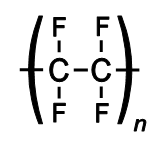
\includegraphics[width=0.2\textwidth]{Teflon_structure.PNG}
			
			\zdroj{GPL, https://commons.wikimedia.org/w/index.php?curid=839743}
			
		\end{frame}
		
		\begin{frame}
		  \frametitle{Historie}
		  \begin{itemize}
		    \item Vynálezci: Wilbert L. Gore a Robert W. Gore 
		    \item Rok: 1969
		  \end{itemize}
		\end{frame}
		
		\begin{frame}
		  \frametitle{Struktura}
		  \begin{itemize}
		    \item 
		  \end{itemize}
		  \begin{figure}
		    \begin{center}
		      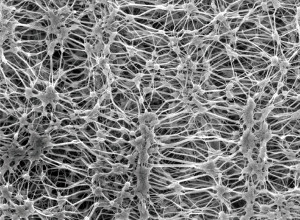
\includegraphics[width=200pt]{membrane_microscopy_small.jpg}
		      \caption{Membrána na snímku z elektronového mikroskopu}
		      \label{fig:membrana}
		    \end{center}
		  \end{figure}
		  \zdroj{http://www.evo.com/waterproof-ratings-and-breathability-guide.aspx}
		\end{frame}
